% begin module first-derivative-up-down
\begin{frame}
\frametitle{What Does $f'$ Say About $f$?}
\begin{columns}[c]
\column{.4\textwidth}
\psset{xunit=1.2cm, yunit=1.2cm}
\begin{pspicture}(-5, -5)(5,5) 
\psframe*[linecolor=white](-5,-5)(5,5) 
\psaxes[ticks=none, labels=none]{<->}(0,0)(-0.5,-0.5)(3.3,2.8)
%Function formula: -5/2-2 ((x) (x))+6 (x) 
\psplot[linecolor=red, plotpoints=1000]{0.381966011}{2.618033989}{x 6 mul x x mul -2 mul add -2.5 add }
%Function formula: -2 (x)+11/2 
\psplot[linecolor=blue, plotpoints=1000]{1.7}{2.3}{5.5 x -2 mul add } %Function formula: 2 (x)-1/2 
\psplot[linecolor=blue, plotpoints=1000]{0.7}{1.3}{-0.5 x 2 mul add } 
\psline[linestyle=dashed](1.5, 2)(1.5, 0)
\tiny
\rput[t](1.5, -0.1){$c$}
\rput[l](0.1, 1.6) {$f'(x)>0$}
\rput[r](2.9, 1.6) {$f'(x)<0$}
\end{pspicture} 
%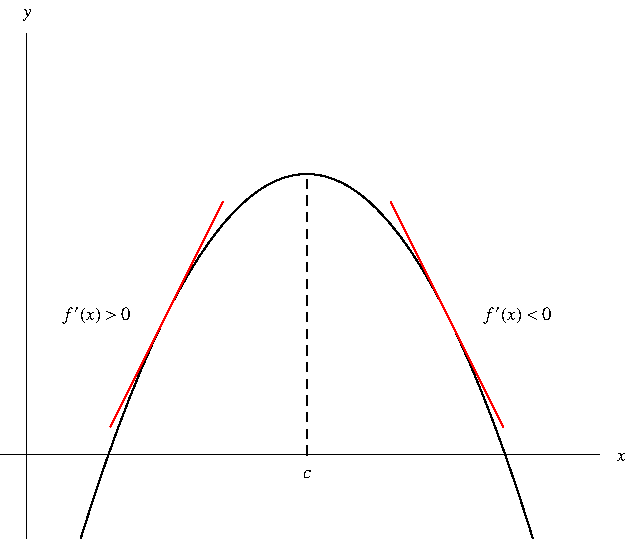
\includegraphics[height=4cm]{curve-sketching/pictures/04-03-firstderiva.pdf}%
\column{.6\textwidth}
\begin{itemize}
\item  Consider the graph on the left. 
\item  $f'(x) > 0$ to the left of $c$ and $f'(x) < 0$ to the right of $c$.
\item  $f$ is increasing to the left of $c$ and decreasing to the right of $c$.
\item<2->  This property holds more generally:
\end{itemize}
\end{columns}
\uncover<2->{Increasing/Decreasing Test}
\begin{enumerate}
\item<2->  If $f'(x) > 0$ on an interval, then $f$ is increasing on that interval.
\item<2->  If $f'(x) < 0$ on an interval, then $f$ is decreasing on that interval.
\end{enumerate}
\end{frame}
% end module first-derivative-up-down